\documentclass[a4paper,10pt,twoside,twocolumn, bg=full]{dndbook} %a4, 10pt, book (idk why i did that...), 2 cols, dnd-themed
\usepackage[english]{babel} %language
\usepackage[utf8]{inputenc} %lovely utf-8
\usepackage{graphicx} %images
\usepackage{wrapfig} %images
\usepackage{array} %allways use this shit, idk why
\usepackage{tikz} %draw stuff
\usepackage{ifthen} %draw stuff
\usetikzlibrary{shapes,calc,fadings} %draw stuff
\usepackage{xspace} %usefull idk, allways import this stuff
\usepackage{dirtytalk} %\say because fuck it
\usepackage{setspace} %don't ask, kind of like it...
\usepackage{pgfplots}

\usepackage[singlelinecheck=false]{caption} %idk dndbook...
\usepackage{listings} %idk dndbook...
\usepackage{shortvrb} %not used yet...
\usepackage{stfloats} %idk dndbook

\singlespacing
\makeatletter %because of titlepage and \HUGE

\@openrightfalse %no empty pages

\graphicspath{{./images/}}

\def \license {GNU Free Documentation License}
\def \licensetext {Please consider and respect the copyleft of this license. The content of this document should be accessible to everyone. Everyone has the right to use the content of this document as he/she wishes, to modify it, to publish it modified (taking into account the copyleft) and to republish it without any changes (taking into account the copyleft).}
\def \author {Sven Hugi}%if you edit this document, add your name... <3
\def \illustrators {} %add name
\def \othercontrib {} %add name

%highlighting with some random effect -> looks handmade and i love it...
\newcommand\hl[2][yellow]{
	\begin{tikzpicture}[
	baseline,
	decoration={random steps,amplitude=1pt,segment length=15pt},
	outer sep=-15pt, inner sep = 0pt
	]
	\node[decorate,rectangle,fill=#1,anchor=text]{#2\xspace};
	\end{tikzpicture}
}
%2 column layout hack...
\newcommand{\nextPage}{%
	\newpage
	\hbox{}
	\newpage
}
%make bad things look ok...
\newcommand{\doublelinebreak}{%
	\linebreak\linebreak
}
%the old HUGE fontsize
\newcommand\HUGE{\@setfontsize\Huge{60}{80}} 

\renewcommand{\maketitle}{%
	\thispagestyle{empty}
	\onecolumn %fuck it
	\vspace*{5cm}
	\begin{center}
		$\vspace*{2cm}$
			{\HUGE\DndFontDropCap{FUESILIER}}\\	
	\end{center}
	\twocolumn %reset shit
}\makeatother
%%%%%%%%%%%%%%%%%%%%%%%%%%%%%%%%%%%%%%%%%%%%%%%%%%%%%%%%%%%%%%%%%%%%%%%%%%%%%%%%%%%%%%%%%%%%%%%%%%%%%%%%%%%%%%%%%%%%%%%%%%%%%%%%%
%											Begin with the document																%
%%%%%%%%%%%%%%%%%%%%%%%%%%%%%%%%%%%%%%%%%%%%%%%%%%%%%%%%%%%%%%%%%%%%%%%%%%%%%%%%%%%%%%%%%%%%%%%%%%%%%%%%%%%%%%%%%%%%%%%%%%%%%%%%%
\begin{document}
	\maketitle
	\section*{Credits}
	\vspace{.25cm}
	\textbf{Author:} \author\linebreak
	%\textbf{Illustrators:} \illustrators\linebreak
	%\textbf{Additional Contributors:} \othercontrib\linebreak
	\textbf{License:} \license\doublelinebreak
	\licensetext\doublelinebreak

	\vfill\pagebreak\hbox{}\vfill\hfill{\tiny This Document was written in \LaTeX.}
	\pagebreak
	\section{Class Features}
		The Füsilier, a light ground troup from the military. Walking around and trying to survive. As the lowest of all, many will think, that you are useless, but in the end, it's the Füsiliers war.
		\begin{DndTable}[header=Füsilier]{cX}
			\textbf{Level}	&\textbf{Features}\\
			$1st$			&\\
			$2nd$			&\\
			$3rd$			& Exhausted Warior, Lightly Armored, Barely Armed\\ % there
			$4th$			&\\
			$5th$			&\\
			$6th$			&\\
			$7th$			& Es steht der Füsilier, Cold Blooded\\ % there
			$8th$			&\\
			$9th$			&\\
			$10th$			& Survival Specialist\\ % there
			$11th$			&\\
			$12th$			&\\
			$13th$			&\\
			$14th$			&\\
			$15th$			& Jack of All Trades\\ % there
			$16th$			&\\
			$17th$			&\\
			$18th$			& Song of Rest\\ % there
			$19th$			&\\
			$20th$			&\\
		\end{DndTable}
		\subsection{Exhausted Warior}
			Starting at level 3, for every level of exhaustion you have, your damage with melee weapon attacks and unarmed strikes is doubbled.
		\subsection{Lightly Armored}
			Starting at level 3 while wearing only light or none armor, you gain a +2 bonus to your stealth checks, dexterity Saving throws and temporary hitpoints equal to your proficiency bonus every turn. You can decide every turn, if you want those temporary hitpoints or not.
		\subsection{Barely Armed}
			Starting at level 3, you are proficient with improvised weapons. Whenever you make a melee attack with a improvised weapon, a pick or a light hammer, you can use your bonus action to make a shove attack.
		\subsection{Es steht der Füsilier}
			Starting at level 7, you can travel for 16h a day, covering doubble of the normal distance. The time you need for a short or long rest is also halved.
		\subsection{Cold Blooded}
			Starting at level 7, you resist cold damage.
		\subsection{Survival Specialist}
			Starting at level 10, you gain proficiency in the survival and nature skill. Difficult terain does not effect your speed and you gain a swimming and climbing speed equal to your walking speed.
			\subsection{Jack of All Trades}
				Starting at level 15, you can add half your proficiency bonus, rounded down, to any ability check you make that doesn't already include your proficiency bonus.
			\subsection{Song of Rest}
Beginning at 18th level, you can use soothing music or oration to help revitalize your wounded allies during a short rest. If you or any friendly creatures who can hear your performance regain hit points at the end of the short rest by spending one or more Hit Dice, each of those creatures regains an extra 1d10 hit points.
	\vfill
	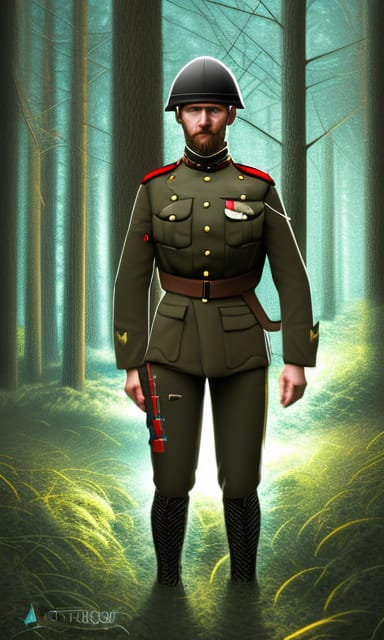
\includegraphics[width=\linewidth]{img.jpg}
	
\end{document}
